\documentclass{standalone}
\usepackage{tikz}
\usepackage{ctex,siunitx}
\usepackage{tkz-euclide}
\usepackage{amsmath}
\usetikzlibrary{patterns, calc}
\usetikzlibrary {decorations.pathmorphing, decorations.pathreplacing, decorations.shapes,}
\begin{document}
\small
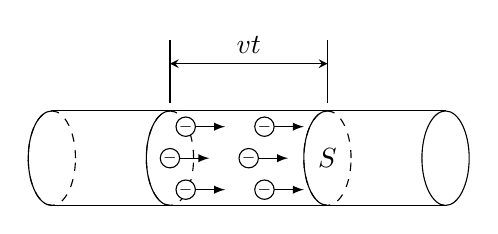
\begin{tikzpicture}[>=latex,scale=1.0]
  \draw(0,.6)--(5,.6);
  \draw(0,-.6)--(5,-.6);
  \draw (5,0) ellipse[x radius=.3, y radius=.6]; 
  \foreach \x in {0,1.5,3.5}
  {
    \draw[dashed](\x,0)ellipse[x radius=.3, y radius=.6]; 
    \draw(\x,.6) arc [start angle = 90, end angle=270, x radius=.3, y radius=.6];
  }
  \node at (3.5,0){$S$};
  \draw(1.5,.7)--(1.5,1.5);
  \draw(3.5,.7)--(3.5,1.5);
  \draw[stealth-stealth](3.5,1.2)--(1.5,1.2)node[midway,above]{$vt$};
  \tkzDefPoints{1.5/0/A, 2.5/0/B, 1.7/-.4/C, 2.7/-.4/D, 1.7/.4/E, 2.7/.4/F}
  \foreach \x in {A,B,C,D,E,F}
  {
    \draw[->](\x)--+(.5,0);
    \draw[fill=white](\x)node{\tiny $-$}circle (3.5pt);
  }
\end{tikzpicture}
\end{document}